\chapter{Model Training}
\label{cha:Main}

\section{Environment Setup}

\subsection{Arena}

The arena used in this thesis can be represented as a $(2 \times 1)m$ surface, on which the obstacles with dimensions $(4 \times 4 \times 16) cm$ are installed. The setup resembles the one used in the thesis of König \autocite{konig2022model} with the distinction that in the current thesis all the obstacles are of one color. To achieve preciseness in measurements, stability and robustness of the material, it was decided to use the 3D-printing technology for the obstacle creating. Such approach also ensures that the process of transferring the setup into the virtual reality goes smoothly, in case there is a need for virtualization. For the first difficulty the obstacles were glued to the surface of the arena to ensure that they'll remain their exact position throughout preparing and evaluation processes. Due to a need in frequent changes in obstacle positions, in the case of second difficulty they were not glued. In every experiment run there are three obstacle pairs installed on the arena. Their position is deliberately chosen to increase the probability that they'd be in the sight of the camera the whole time before the robot passes them.

\subsection{Hardware}

To collect the training data and test the trained models we use the same JetBot by NVIDIA that was used in previous works from ScaDS.AI. It has $4$ GB of video-memory and $128$ CUDA-cores that are able to operate at the maximum of $921$ MHz clock speed. These computational abilities are enough for the system to be able to execute the final control prediction pipeline at the frequency of $4$ times per second. As for the moving part, it consists of 2 electro-motors connected to the computing unit. To control the mechanical part of the robot we used the JetBot API, which very conveniently has Python bindings. There are multiple modes in which one could operate the JetBot, but the most straightforward approach, which was used in this thesis, is to directly set the speeds of the motors to values in range $[-1,1]$.

\subsection{Software}
For the simplicity of making frequent changes to the model architecture, it was decided to use the Keras framework for Python programming language. This is a high-level framework that was built on top of existing Tensorflow library, which encapsulates all the GPU-computations and low-level details, simplifying the development to machine learning models. The main reasoning for choosing this framework were the simplicity of the syntax and a large quantity of ready-to-use layers, activation functions, learning optimizators etc. It also comes with very convenient toolset for neural network training, that includes embedded data augmentator for image datasets. Unfortunately, since dealing with the data sequences, which need to be handled very specifically in order to train the model using the right framerate, a custom data augmentation pipeline was developed.

There was a problem in matching the versions of tensorflow between different devices. The Jetson hardware supports only a particular version of cuDNN, which is required for Tensorflow. Therefore, there was a need in downgrading the version of the library for the whole project.

For dealing with large arrays and performing fast computations on matrices a NumPy Python library was utilized. It comes with a large number of mathematical functions that execute the compiled C++ code underneath, which gives such dynamic language as Python the fast computational advantages of native programming languages.

All the operations that were performed on images were done using the OpenCV Python library. This library comes with a large quantity of methods to transform, modify and store the image data. It was a very useful tool throughout the whole work on the thesis.

\section{Data Acquisition}

To be able to perform supervised training on a demonstration data (Behavioral Cloning), a labeled dataset needed. The dataset $D$ is represented as a vector where each entry $(x_i, y_i) \in D$ is a tuple, where $x_i$ is the data obtained from the sensors (camera input) and $y_i$ is the vector that represents the controls required for the vehicle to move at the current point in time. In this case, a gamepad was used to be able to collect the data and specifically the inclination of it's left stick are used to calculate the motor speeds of the JetBot. Specially for the acquisition part, a special software pipeline was developed, the main purpose of which was to enable the control of the vehicle, collection of data from the sensors and storing the collected data. The pipeline consists of two software components: \textit{server}, which is executed on the JetBot itself, and \textit{client}, which is executed on any other machine connected to the same network as JetBot. The developed pipeline works as follows:

\begin{enumerate}
  \item The server program on the JetBot is started. It consists of two separate threads.
  \item In one thread the OpenCV video capturing pipeline is started.
  \item In another thread a TCP server starts listening for a new connection on a particular port. Python's internal socket library was used to perform all the network operations.
  \item On another machine the client software is launched. This program ensures that the gamepad is connected to the machine. To obtain information about connected devices and listen for controlling inputs from the gamepad the Pygame library was used.
  \item When the connection is established, the server on JetBot awaits the input data from the port in a loop.
  \item Upon receiving the first controlling input from the gamepad the client software starts continuously sending the current position of the gamepad's stick to the server.
  \item Once the new data is received in the TCP-server-thread, the variable that is shared between both threads is updated.
  \item Once the video-thread captures a new frame, it is stored on the device. Then it checks for the updates in the controlling input's variable and then derives the motor inputs from this data. For a gamepad's stick position represented as $(x, y)$, the inputs for left and right motors are calculated as follows in the algorithm \ref{alg:motor_inputs}.
  \item Using JetBot API the values are passed to the motors and the cycle continues until the termination of the program.
  \item When the program is terminated, a process of transferring all of the sensor data from the JetBot to the client is started.
  \item At the moment the data transfer is finished, all the video frames are stored in a separate directory. The controlling sequence is stored in the same directory in a default format used by the NumPy Python library. The controls data is represented as a sequence of tuples $(x, y, t)$, where $x$ and $y$ encode gamepad's stick position and $t$ is the time in milliseconds from the start of the run.
\end{enumerate}

\begin{algorithm}
  \caption{Calculation of motor inputs based on the gamepad's stick position}
  \begin{algorithmic}[1]
    \Function{CalculateMotorInputs}{$x, y$}
    \State $\text{rotation\_quotient} \gets 0.5$
    \State $left\_power \gets -y + x \cdot \text{rotation\_quotient}$
    \State $right\_power \gets -y - x \cdot \text{rotation\_quotient}$
    \State $max\_power \gets \max\left( \left|left\_power\right|, \left|right\_power\right|, 1 \right)$
    \State $left\_power \gets left\_power / max\_power$
    \State $right\_power \gets right\_power / max\_power$
    \State \Return $left\_power, right\_power$
    \EndFunction
  \end{algorithmic}
  \label{alg:motor_inputs}
\end{algorithm}

The data was firstly collected using smaller frame rates (30FPS), but then it was decided to increase the frequency to 120FPS. The reasoning behind this was that, although the system is not able to execute the agent on such high frequencies, the frame sequence could be split while training and it would be possible to train the model using the frequency that suits the conditions.

Once all the data is collected, it should have ben filtered in the way that all the bad (unrepresentative) trajectories are deleted and the good trajectories are cropped to remove the data points that could obstruct the learning process of feature extraction. In particular, the image sequence that followed after the the JetBot crossing the last obstacle pair was completely deleted since it didn't contain any useful demonstration data.

The final dataset consists of $22017$ labeled images and is split into 2 parts: first difficulty and second difficulty. It must be said that the quality of the data for the second difficulty is not as good as for the first one and the quantity of the data is too small even for the first difficulty. The first difficulty part consists of $15008$ data-points and the rest if the second difficulty. Considering that the second difficulty requires a lot more generalizability from the model than the first one, the dataset for the second difficulty should've contained more data and it should've been more diverse and with better feature distribution variance. Due to time restrictions, the amount of work load that this thesis required and the time-consuming and difficult process of obtaining and filtering new data, it was decided to continue the training process using the existing dataset.

\section{Data Pre-processing}

Before starting the training with the data that was collected, the next step is to pre-process it to make training more effective and to reduce the amount of noise that the model could mishandle for a feature. The preprocessing steps for the images that were used in the final iteration of the model training process are as follows:

\begin{enumerate}
  \item \textbf{Gray-scaling} \\
    There is a hardware restriction on the time and space complexity of the agent that we're able to run on the JetBot. Thus, the size of the model and it's computational time have a big impact on the frequency with which the model will be able to predict the controls. For this purpose, all the images are gray-scaled before passing them into the network. The formula $Y = 0.299 \times R + 0.587 \times G + 0.114 \times B$, where $R$, $G$ and $B$ are the matrices of the red, green and blue components of the image respectively, was used to perform the gray-scaling operation.
  \item \textbf{Pixel-centering} \\
    For the CNN to achieve a good accuracy, it's not enough to train it on the raw data. As the experiments show \autocite{pal2016preprocessing}, the CNNs perform much better if the data they are fed is normalized in some way. In the final iteration of the agent all the images that are used as an input for the neural network are centralized right before passing them into the neural network using formula $Y_c = Y / 127.5 - 1$, where $Y$ is the gray-scaled image matrix.
  \item \textbf{Region of Interest} \\
    The region of interest  is cropped out of each image. This is done to reduce the dimensionality of the network, so that the computations are faster, and to increase the percentage of pixels that are important for feature extraction on the image.
\end{enumerate}

\subsection{Edge detection}
\label{sec:edge-detection}

Despite the pre-processing steps being straightforward and not convoluted in the final iteration of the agent, a huge work was done on experimenting with different approaches and figuring out, what works the best.

Farag et al. \autocite{8855753} came up with a sound future work proposition in their work: to utilize edge detection mechanism on an image before passing it into the CNN. On an intuitive level this approach would enable the CNN to be able to derive features from images more easily, since all the objects would be more distinguishable. Theoretically it would simplify the task of selecting obstacles on the way of the robot, so that the model would be able to lean to derive more complex and meaningful for the task features faster. Two edge detection algorithms were tested: one of them was the Canny edge detector \autocite{canny1986computational}, as proposed in \autocite{8855753}, another one was the Sobel filter \autocite{sobel2014history}. After training and experimenting with the models trained using both these approaches, there were no signs that edge detection would somehow help the model better generalize more complex features. The best results that could be obtained using edge detectors were for the JetBot to stably pass the second pair of obstacles and then fail to pass the third one. The first model trained on data that did not go through the process of edge detection has shown great performance improvement in comparison to it's predecessors. The main reason for such poor performance could be that the algorithms are very noise-prone. Although methods such as Gaussian blurring were used to smooth the images and decrease noise level, the algorithms still produced artifacts that the model was very likely to mismatch for a feature.

Despite edge detection being a very promising technique, the training was not able to achieve any good results using this approach. Another interesting development possibility was was to use Quantized Neural Network (QNN). In this method all the weights are represented as either integer values or even single-digit binary values. Since Canny edge detector algorithm produces binary matrix, it would've been possible to develop a quantized CNN that would derive features from such matrix. Such approach would drastically lower the size of the model and increase the computational speed, since integer-valued operations cost less computing cycles than operations with the floating point.

\section{Model Architecture}

One of the main tasks of this thesis was to develop an architecture of the CNN that would be able to learn to extract sufficient features from the image sequence data. Before starting the development of the architecture it had already been established that the model will have to be able to extract not only spacial features from the image, but also temporal features from the sequence of previous images. It has lead to the necessity to use a concept of memory stack \autocite{schneeberger2024end} \autocite{schaller2023train}.

Different configurations and approaches were tested to find the best model architecture that would be able to learn to extract features under the constraint of the poor quality of the data. In the scope of this work, tens of model architectures and their configurations were trained. Many of them didn't prove to be efficient in the task solving and were immediately put aside after testing. Here is the listing of the most performative models:

\begin{enumerate}
  \item \textbf{Previous theses' approach:} \\
    The approach of Schneeberger \autocite{schneeberger2024end} and Schaller \autocite{schaller2023train} consisted of using the convolutional channels to process the sequence --- one channel per image. For this purpose, the CNN model from the OpenAI's Stable Baselines 3 (the same model that was used in \autocite{schneeberger2024end}) was replicated using Keras (originally it was implemented in PyTorch) and slightly corrected to fit the dimensional requirements. The architecture is depicted in figure \ref{fig:sb3cnn-arch}.
    \begin{figure}[htbp]
      \centering
      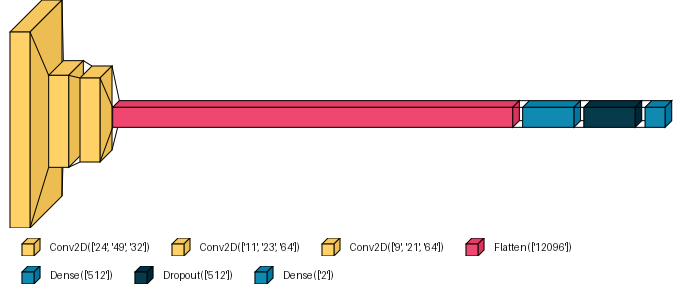
\includegraphics[width=0.8\textwidth]{Images/SB3CNN_architecture.png}
      \caption{Architecture diagram of the CNN model from Stable Baselines 3.}
      \label{fig:sb3cnn-arch}
    \end{figure}
    The model didn't show well during the training --- because of the absence of improvement in the validation loss, the training was terminated automatically by the Early Stopping mechanism already on epoch $10$.
  \item \textbf{DAVE-2:} \\
    The architecture used by researchers from NVIDIA in \autocite{bojarski2016endendlearningselfdriving} was replicated exactly as it is in the paper. This is the only model that was used in this thesis that didn't use any kind of memory mechanism and simultaneously the only model that didn't require any kind of preprocessing to be done, except for image cropping. The model takes the raw image as an input (3-channeled input layer is used to process red, green and blue components of the image). The architecture is demonstrated in figure \ref{fig:dave-2-arch}.
    \begin{figure}[htbp]
      \centering
      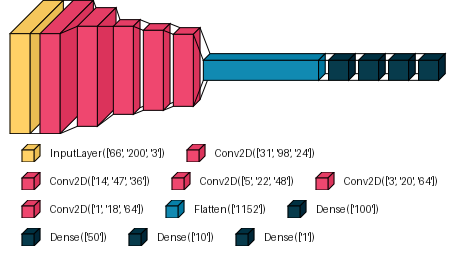
\includegraphics[width=0.5\textwidth]{Images/DAVE-2_architecture.png}
      \caption{DAVE-2 architecture.}
      \label{fig:dave-2-arch}
    \end{figure}
  \item \textbf{BCNet with LSTM:} \\
    BCNet is the name of the architecture used in \autocite{8855753}. It resembles DAVE-2 in many ways, but has some significant distinctions (number of layers and layer sizes). The goal in \autocite{8855753} was to develop a model that would predict the steering angle of the vehicle. Certain corrections had to be made in order to fit this model into the setting of current thesis --- including dimensional changes in layers, output etc. Farag et al. \autocite{8855753} proposed multiple possible improvements for their system, including usage of Long Short-Term memory (LSTM) layers and edge detection mechanism for images before passing them into the CNN. As already stated in \autoref{sec:edge-detection}, edge detection hasn't proven to be a working solution that would somewhat improve the network's feature extraction abilities.

    The architecture of the model is illustrated in figure \ref{fig:BCNet-LSTM-arch}. In order to be able to combine the LSTM and normal architecture in one model, the the usage of Time Distributed layers from Keras was involved. These layers enable to perform transformation using convolutional layers on each of the images in the data sequence separately and then pass the transformed sequence to the LSTM in one batch.
    \begin{figure}[htbp]
      \centering
      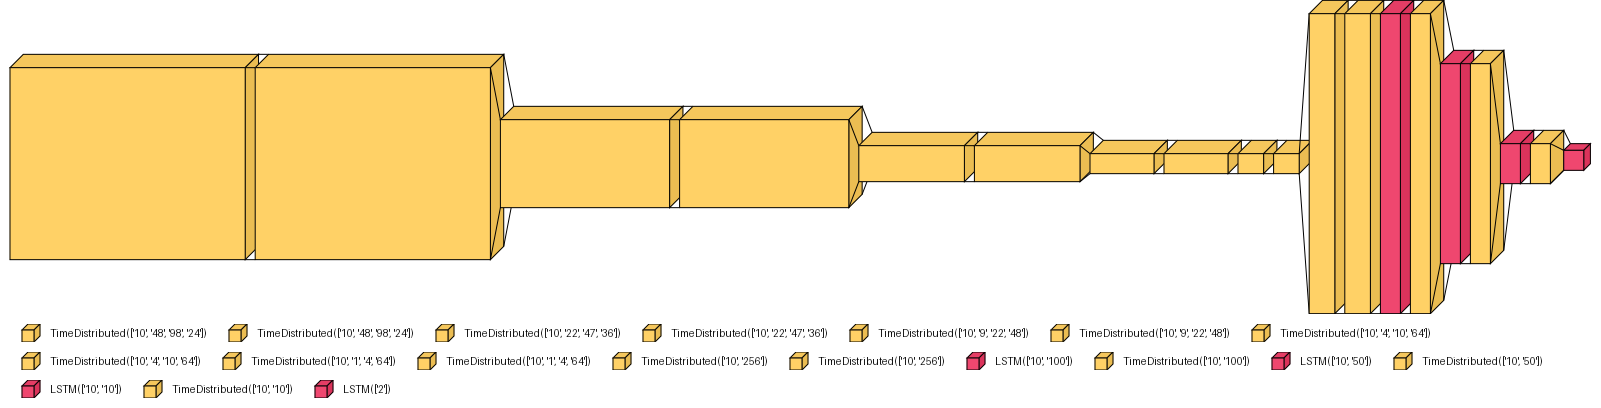
\includegraphics[width=0.9\textwidth]{Images/BCNetLSTM_architecture.png}
      \caption{BCNet with LSTM layers. The Time Distributed layers represent the Convolutional, Flattening and Dropout layers of the network.}
      \label{fig:BCNet-LSTM-arch}
    \end{figure}
\end{enumerate}

The detailed explanation of performance testing and comparison between models is described in \autoref{cha:Evaluation}.

% TODO: model architecture, model diagram, image preprocessing diagram